\chapter{ORB-SLAM在家居设计和增强现实中的应用构想}

\section{ORB-SLAM方法简述}

ORB-SLAM \cite{Mur-Artal2015}
是近几年比较火热的单目相机的SLAM方法,它在PTAM的基础上采用了效率更高的特征提取和优化算法,改进了PTAM的双进程为三进程,加入闭环检测(loop closing),并优化了代码结构,使得该算法较PTAM更稳定,更实用,也更有移植到移动端的潜力。

该算法的流程如\autoref*{fig:ORBprocess}所示,算法主要维护三个进程:追踪进程(Tracking)与PTAM类似,主要用于相机姿态的估计,但不同的是采用了比FAST更优的ORB \cite{Strasdat2011}
特征点提取方法,同时改进了关键帧的判定。局部映射进程(Local Mapping)则与PTAM中的映射进程类似,在有了新的关键帧之后,算法需要维护关键帧集合,构建重建信息,同时进行BA优化。ORB-SLAM算法维护的第三个进程,即闭环检测进程(loop closing),利用了DBoW2\cite{Galvez-Lopez2012}技术,通过构建词典检测图片序列中的语义场景,从而判定相机轨迹中是否存在闭路的情形,
同时对检测到的闭路进行优化,提高追踪精度并减少重复计算。

为了降低全局的时间复杂度,ORB-SLAM维护一个基于关键帧到关键帧的图结构(Covisibility Graph)
\cite{Galvez-Lopez2012}
,用图模型中边的权值(共享特征点数量)衡量关键帧的相似度,同时取稠密图中的MST(Essential Graph)作为子图实际参与优化,在保证鲁棒性的前提下尽可能提高效率。


\begin{figure}[!htbp]
\centering
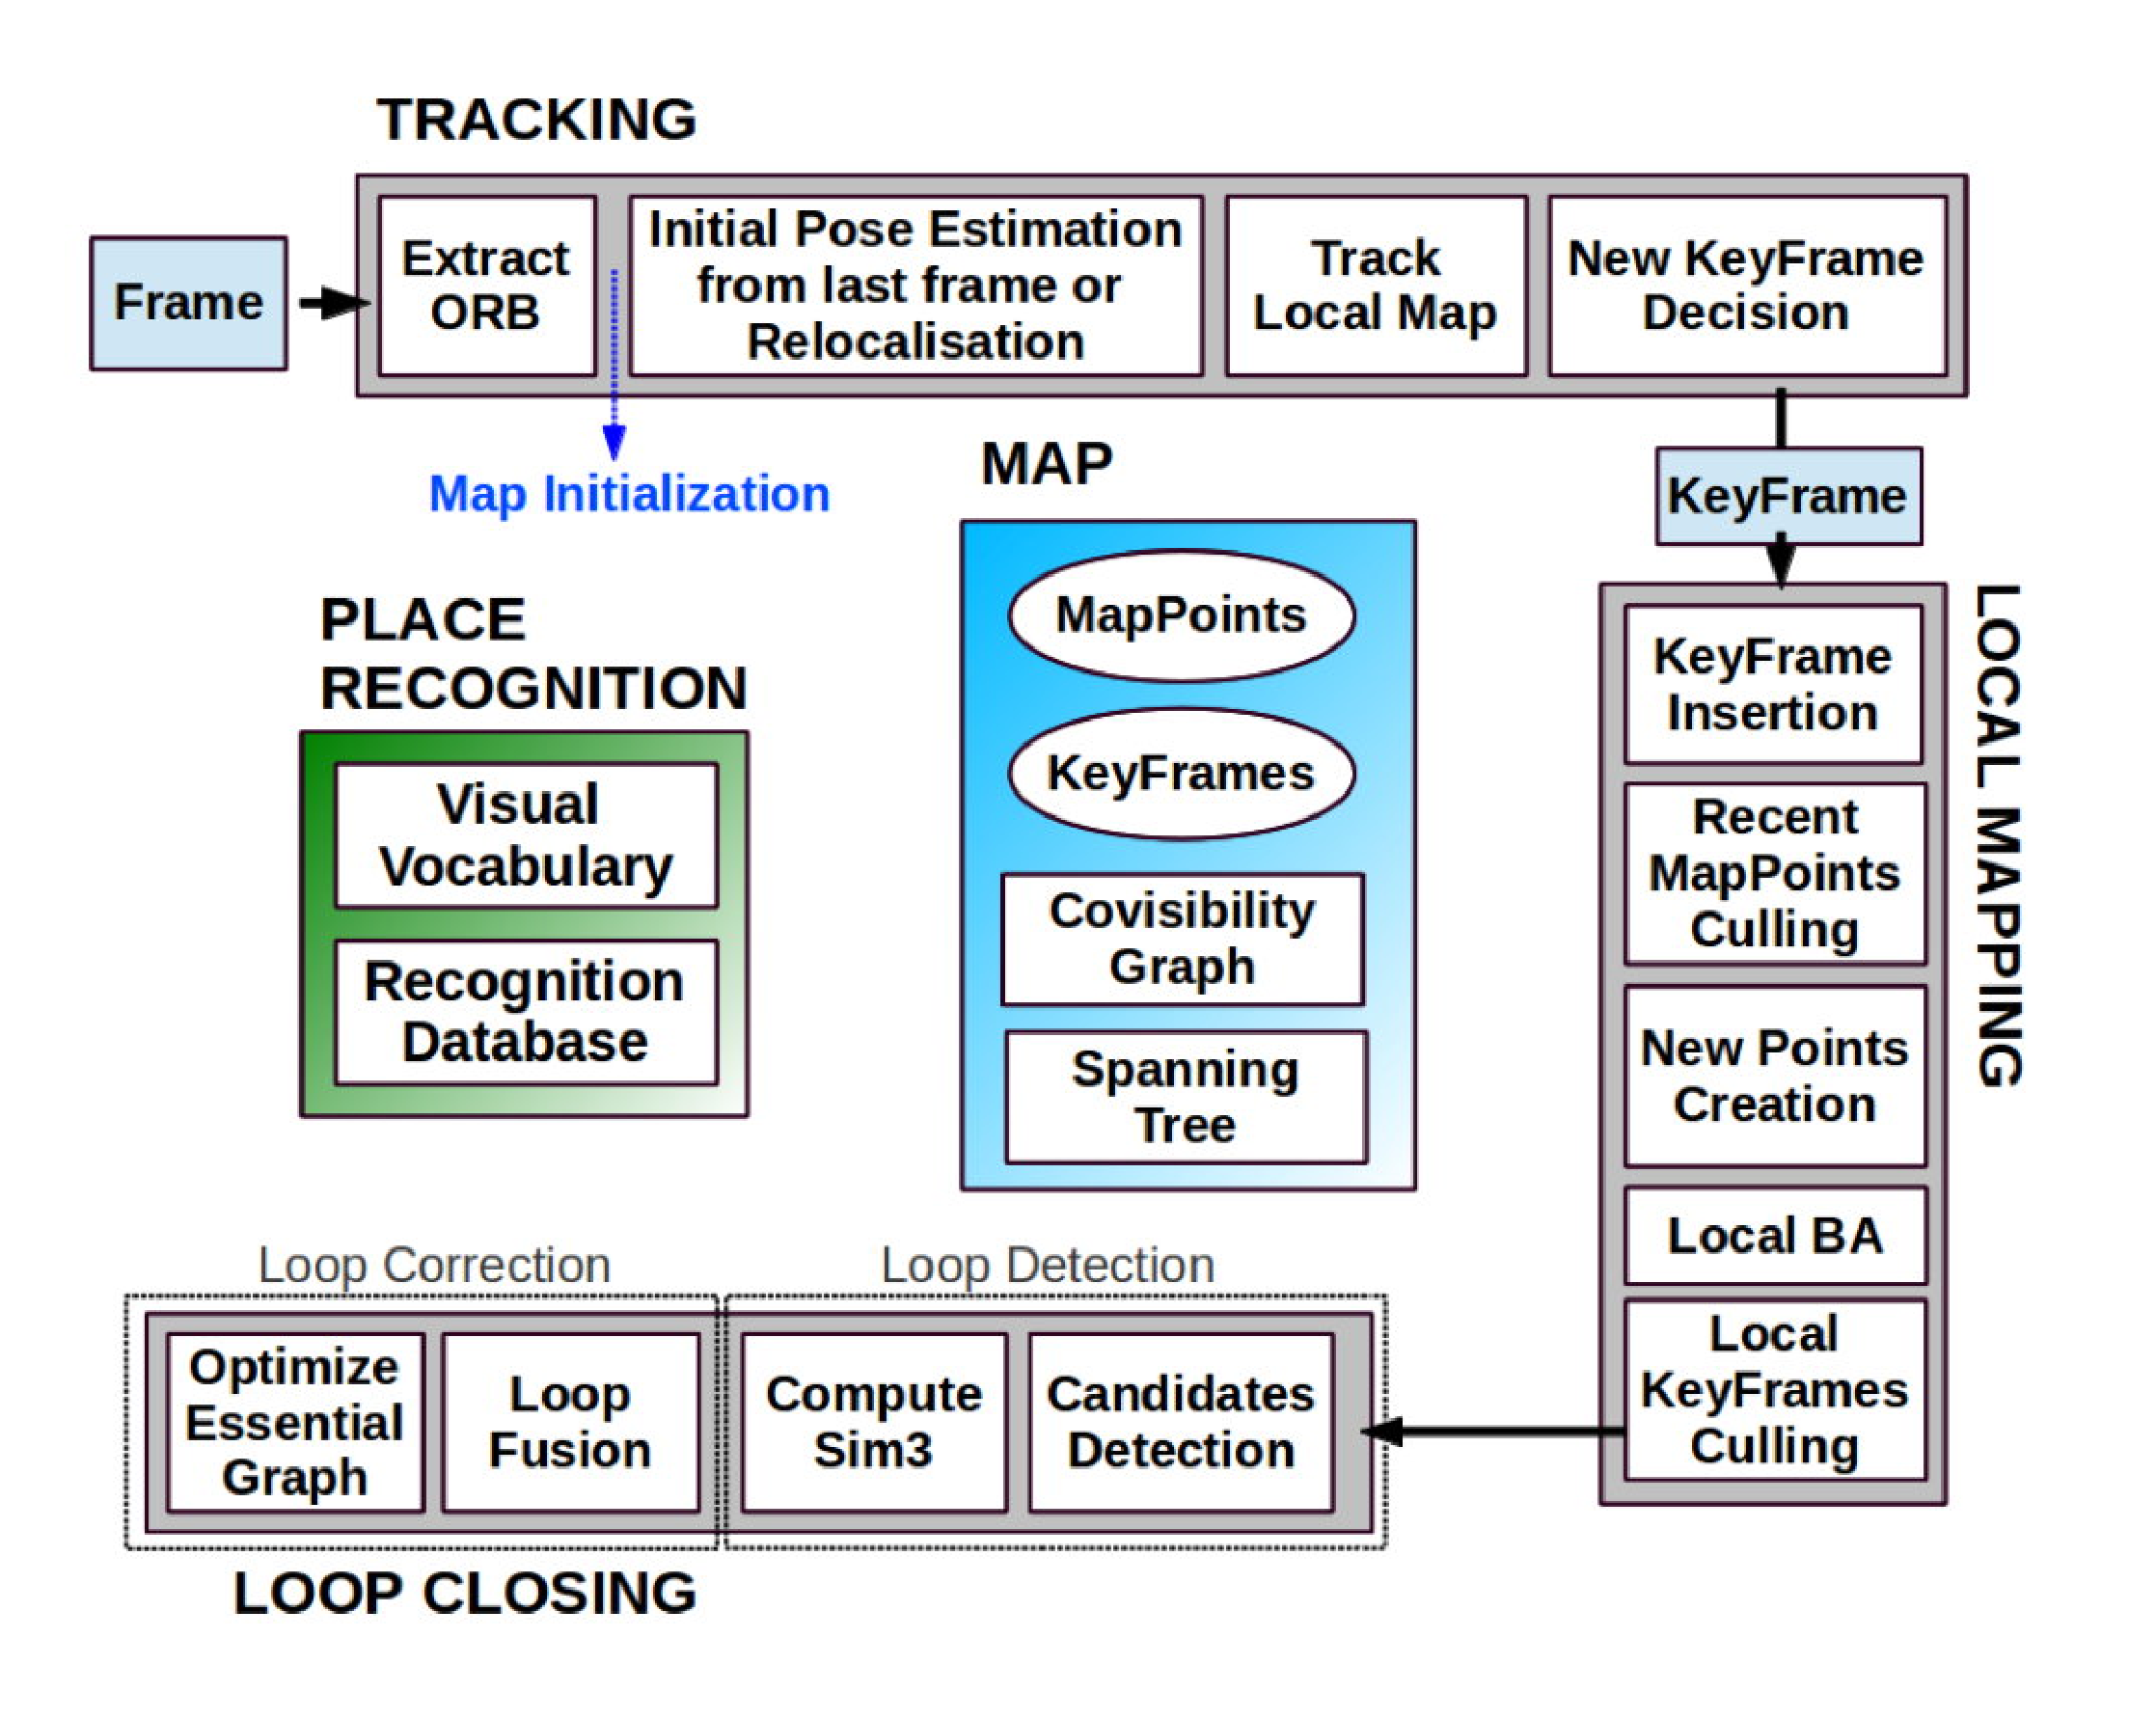
\includegraphics[width=12cm]{ORBSLAM.pdf}
\caption{ORB-SLAM算法的主要流程示意}
\label{fig:ORBprocess}
\end{figure}

